\section{Further Topics in Analytic Number Theory}
Recall the observation in the very first chapter that the number of digits in the error approximating $\pi(x)$ by $\textrm{Li}(x)$ was approximately half that of $x$. However, the error term we proved in the prime number theorem is not quite of the order $x^{1/2}$. So, is it possible to improve this? Note that the error term effectively corresponds to how good the zero-free region of $\zeta(s)$ is. With more advanced methods, introduced by Vinogradov and Korobov \cite[Chapter~6]{ivic_2003}, one can prove a slightly sharper zero-free region, 
\begin{equation}
    \sigma \geq 1 - C(\log t)^{-2/3} (\log \log t)^{-1/3} \nonumber
\end{equation}
for an absolute constant $C$. Using this zero-free region, one can prove as in \cite[Chapter~12]{ivic_2003} that
\begin{equation}
    \pi(x) = \textrm{Li}(x) + O\left(x \exp\{-C(\log x)^{3/5}(\log \log x)^{-1/5} \} \right). \nonumber
\end{equation}
Now, it would not be a report about analytic number theory without mentioning the Riemann Hypothesis (RH). In his 1859 memoir, Riemann conjectured that every non-trivial zero of $\zeta(s)$ lies on the `critical line', $\sigma = 1/2$. Assuming this gives essentially the strongest possible version of the prime number theorem, which we show using the method from \cite[p.~113]{davenport}. Starting with the explicit formula (\ref{ExpicitPsiFormula}), we have for $T \geq 2$,
\begin{equation}
    \psi(x) = x - \sum_{\abs{\rho} < T} \frac{x^{\rho}}{\rho} + O\left( \frac{x \log^{2} x} {T} \right). \nonumber
\end{equation}
Then, since necessarily $\abs{x^{\rho}} = x^{1/2}$, and $\sum_{\abs{\rho} < T} \frac{1}{\rho} = O(\log^{2} T)$, we set $T = x^{1/2}$ to give
\begin{align}
    \psi(x) &= x + O(x^{1/2} \log^{2} x), \nonumber \\
    \pi(x) &= \textrm{Li}(x) + O(x^{1/2} \log^{2} x). \nonumber
\end{align}
Note that this coincides with our observation that the error was approximately of order $x^{1/2}$! Therefore, a proof of the Riemann Hypothesis would give us the ability to give highly accurate estimates of how many primes there are less than a given value. As of yet, sadly, no such proof has been found despite the best efforts of some of the very best mathematicians. There is a much stronger analogous hypothesis in the case of Dirichlet L-functions, namely that all L-functions also have all their non-trivial zeros on the critical line - known as the Generalised Riemann Hypothesis (GRH). This then gives the same error estimate for $\pi(x; q, a)$ under GRH as for $\pi(x)$ under RH (only subject to the condition that $q \leq x^{1/2}$!) \cite[p.~124]{davenport}. \\

We now return to the `bias' of primes to certain residue classes which was alluded to at the end of the previous section, and use data and results from \cite{granville2004prime}. Our aim is to pit the different arithmetic progressions of a given modulus against each other in a `prime number race'. As a first example, consider the primes mod $4$. With the exception of $2$, primes are either congruent to $1$ or $3$ modulo $4$, and by the prime number theorem for arithmetic progressions, we have
\begin{equation}
    \pi(x; 4, 1) \sim \pi(x; 4, 3) \sim \frac12 \textrm{Li}(x). \nonumber
\end{equation}
Now, let us consider the empirical evidence.
\begin{table}[H]
    \centering
    \begin{tabular}{|c|c|c|}
        \hline
        $x$ & $\pi(x; 4, 3)$ & $\pi(x; 4, 1)$ \\
        \hline
        100 & 13 & 11 \\
        200 & 24 & 21 \\
        300 & 32 & 29 \\
        400 & 40 & 37 \\
        500 & 50 & 44 \\
        1000 & 87 & 80 \\
        \hline
    \end{tabular}
    \caption{A comparison of $\pi(x; 4, 3)$ and $\pi(x; 4, 1)$}
\end{table}
Despite growing at the same rate, $\pi(x; 4, 3)$ `stays ahead in the race' against $\pi(x; 4, 1)$. Or, more formally $\pi(x; 4, 3) - \pi(x; 4, 1)$ stays positive for every value of $x$ shown. Is this mere coincidence? Let us consider $\pi(x; 4, 3) - \pi(x; 4, 1)$ plotted over many more values of $x$ in the figure below\footnote{Plot made using Python 3.7.4 and the library Seaborn 0.10.0.}. Remarkably, $\pi(x; 4, 3)$ stays ahead for all but one of the first $100,000$ values. 
\begin{figure}[H]
    \centering
    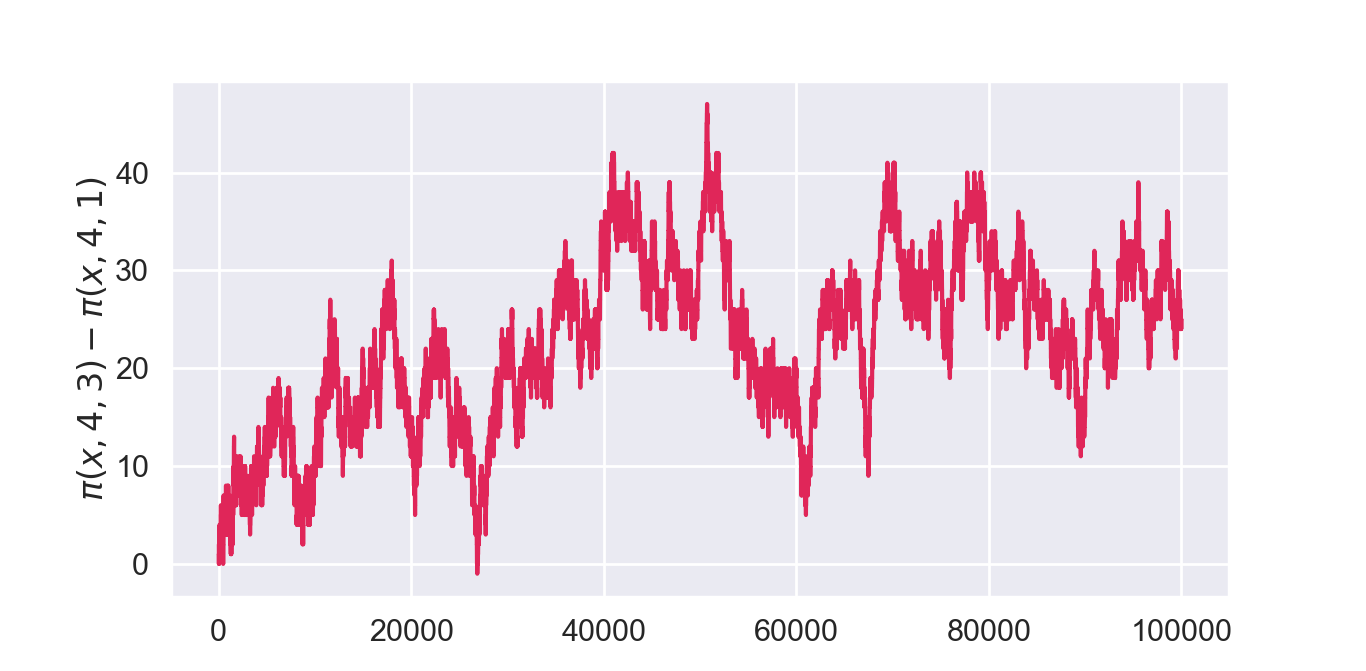
\includegraphics[width=0.7\textwidth]{Chapter5/prime_race_4.png}
    \caption{The difference $\pi(x; 4, 3) - \pi(x; 4, 1)$ for $0 \leq x \leq 10^{5}$}
\end{figure}
This bias in favour of the form $4n + 3$ among primes is known as Chebyshev's bias, who first remarked upon it. However, $\pi(x; 4, 3)$ does not always stay ahead in this race. In fact, Littlewood (1914) showed that $\pi(x; 4, 3) - \pi(x; 4, 1)$ changes sign infinitely often. Despite this, the first time that $\pi(x; 4, 1)$ takes the lead is at $x = 26,861$, before immediately losing it at $x = 26,863$! The case of modulus $4$ is by no means an isolated case either. Indeed, consider the mod $10$ race (the last digit of the primes). Numbers coprime to $10$ are $1$, $3$, $7$ and $9$, so consider the growth of the number of primes in these arithmetic progressions.
\begin{table}[H]
    \centering
    \begin{tabular}{|c|c|c|c|c|}
    \hline
       $x$ & $\pi(x; 10, 1)$ & $\pi(x; 10, 3)$ & $\pi(x; 10, 7)$ & $\pi(x; 10, 9)$ \\
       \hline
        100 & 5 & 7 & 6 & 5 \\
        200 & 10 & 12 & 12 & 10 \\
        500 & 22 & 24 & 24 & 23 \\
        1000 & 40 & 42 & 46 & 38 \\
        2000 & 73 & 78 & 77 & 73 \\
        5000 & 163 & 172 & 169 & 163 \\
        10,000 & 306 & 310 & 308 & 303 \\
        20,000 & 563 & 569 & 569 & 559 \\
        50,000 & 1274 & 1290 & 1288 & 1279 \\
        100,000 & 2387 & 2402 & 2411 & 2390 \\
        \hline
    \end{tabular}
    \caption{The mod 10 prime race for values up to $10^{5}$}
\end{table}
The pattern here is perhaps less easy to see, but after some examination we spot that the two middle columns seem to remain slightly ahead - there is essentially a small bias towards primes with a last digit of $3$ and $7$ compared to $1$ and $9$. So, why do these biases occur? Another prime race helps to reveal the pattern, namely the mod $8$ race. 
\begin{table}[H]
    \centering
    \begin{tabular}{|c|c|c|c|c|}
    \hline
        $x$ & $\pi(x; 8, 1)$ & $\pi(x; 8, 3)$ & $\pi(x; 8, 5)$ & $\pi(x; 8, 7)$\\
        \hline
        1,000 & 37 & 44 & 43 & 43 \\
        5,000 & 161 & 168 & 168 & 171 \\
        10,000 & 295 & 311 & 314 & 308 \\
        50,000 & 1,257 & 1,295 & 1,292 & 1,288 \\
        100,000 & 2,384 & 2,409 & 2,399 & 2,399 \\
        1,000,000 & 19,552 & 19,653 & 19,623 & 19,669 \\
        \hline
    \end{tabular}
    \caption{The mod 8 race for values up to $10^{6}$}
\end{table}
There is no clear winner in this race, but there is a clear loser - namely primes of the form $8n + 1$. So far, the losers in the races have been
\begin{itemize}
    \item $1$ mod $3$,
    \item $1$ and $9$ mod $10$,
    \item $1$ mod $8$.
\end{itemize}
Now, these residue classes are precisely the quadratic residues that lie in the multiplicative group of each modulus. This gives us a heuristic idea for why these biases occur: numbers in the progressions corresponding to quadratic residues are somehow `less likely' to be prime, as \textit{all} the squares of primes lie in these residue classes. So, what results have been proved (or disproved) relating to this phenomenon? These biases were studied comprehensively in a paper of Rubinstein and Sarnak (1994) \cite{Rubinstein1994ChebyshevsB}. A big conjecture in this area was that of Knapowski and Turán (1962) \cite[p.~3]{granville2004prime}:
\begin{conjecture}
As $X \rightarrow \infty$, 
\begin{equation}
    \frac{1}{X} \#\{x \leq X \ \textrm{s.t.} \ \pi(x; 4, 3) - \pi(x; 4, 1) > 0 \} \rightarrow 1. \nonumber
\end{equation}
\end{conjecture}
In essence, this states that Chebyshev's bias holds for almost all values of $x$. Although empirical evidence suggests this conjecture may be true, it was disproved by Sarnak and Knapowski independently (1994 and 1993 respectively). However, Rubinstein and Sarnak had the idea of counting $1/x$ for each $x \leq X$, rather than simply $1$. Then, since $\sum_{x \leq X} x^{-1} \approx \log X$, we normalise by a factor of $\log X$ rather than $X$. Their inspired idea had the following result \cite[p.~18]{granville2004prime}:
\begin{equation}
    \frac{1}{\log X} \sum_{\substack{x \leq X \\ \pi(x; 4, 3) - \pi(x; 4, 1) > 0}} \frac{1}{x} \rightarrow 0.9959\dots \ \textrm{as} \ X \rightarrow \infty. \nonumber
\end{equation}
To count the bias in this way is termed the `logarithmic measure'. Thus, instead of Chebyshev's bias holding almost always, it actually holds approximately $99.59\%$ of the time! The way this result was derived relies heavily on results we proved regarding Dirichlet L-functions. The caveat to this result, is that it relies on two (as of yet) unproven conjectures. The first is GRH, while the other is known as the Grand Simplicity Hypothesis, which states that all the zeros on the critical line are linearly independent. They also argued in greater generality than just the case of $q = 4$. Indeed, they proved that if $a, b$ are coprime to $q$, with $a$ a square mod $q$ and $b$ not square, then a bias necessarily exists towards $b$, but holds less than $100\%$ of the time. More precisely, there exists $1/2 < c < 1$ such that
\begin{equation}
    \frac{1}{\log X} \sum_{\substack{x \leq X \\ \pi(x; q, b) - \pi(x; q, a) > 0}} \frac{1}{x} \rightarrow c \ \textrm{as} \ X \rightarrow \infty. \nonumber
\end{equation}
Moreover, they proved that if $a$ and $b$ are either both squares or both non-squares mod $q$, then no such bias exists, and this limit is exactly $1/2$. In a nutshell, there is a bias if and only if exactly one of $a$ and $b$ is a quadratic residue. These biases may also be studied in greater generality: more recent work by Lemke Oliver and Soundararajan (2016) \cite{LemkeOliverE4446} studied biases in \textit{sequences} of primes in arithmetic progressions. They observe that the size of the biases between different tuples of reduced residue classes can be even more vast. As a basic example, consider the last digits of all pairs of consecutive prime numbers (the case of modulus $10$). We define
\begin{equation}
    \pi(x; 10, (a, b)) = \#\{p_n \leq x \ \textrm{s.t.} \ p_n \equiv a \ (10) \ \textrm{and} \ p_{n+1} \equiv b \ (10) \}. \nonumber
\end{equation}
Then, if $x_0$ is such that $\pi(x_0) = 10^{8}$, we have the following data for $\pi(x_0; 10, (a, b))$.
\begin{table}[H]
    \centering
    \begin{tabular}{|c|c|c|c|c|}
    \hline
        & $a=1$ & $a=3$ & $a=7$ & $a=9$ \\
        \hline
        $b=1$ & 4,623,042 & 6,010,382 & 6,373,981 & 7,991,431  \\
        \hline
        $b=3$ & 7,429,438 & 4,442,562 & 6,755,195 &  6,372,941  \\
        \hline
        $b=7$ & 7,504,612 & 7,043,695 & 4,439,355 &  6,012,739  \\
        \hline
        $b=9$ & 5,442,345 & 7,502,896 & 7,431,870 &  4,622,916  \\
        \hline
    \end{tabular}
    \caption{The value of $\pi(x_0; 10, (a, b))$ for different values of $a$ and $b$, where $\pi(x_0) = 10^{8}$}
\end{table}
Notice the fact that the diagonals are vastly different from the other numbers in the table: essentially, if you pick a prime at random less than $x_0$, the chance that the next prime will have the same digit is actually much smaller than $25$ percent! This phenomenon was explained only heuristically in \cite{LemkeOliverE4446}, and relies on the Hardy-Littlewood k-tuples conjecture, which is essentially a result of the type of the prime number theorem but for arbitrary sequences of primes. To give an idea of the strength of this conjecture, one special case is a strengthening of the (as of yet unproven) twin prime conjecture, which states there are infinitely many primes that are $2$ apart. The study of these biases in sequences of primes less than a given value therefore `blur the lines' between problems of global and local type - a broad categorisation of problems relating to the primes which we discussed earlier. We shall not go into the details of the results of \cite{LemkeOliverE4446}, as they are beyond the level of this report. In summary, we have now explored the data relating to primes in arithmetic progressions, and given even more detail regarding their behaviour in specific residue classes. This is in stark contrast to the result of the prime number theorem for arithmetic progressions, which makes no distinction between different residue classes of a given modulus. 